%% 美赛模板:正文部分

\documentclass[12pt]{article}  % 官方要求字号不小于 12 号,此处选择 12 号字体

% 本模板不需要填写年份,以当前电脑时间自动生成
% 请在以下的方括号中填写队伍控制号
\usepackage[2506135]{easymcm}  % 载入 EasyMCM 模板文件
\problem{C}  % 请在此处填写题号
\usepackage{mathptmx}  % 这是 Times 字体,中规中矩 
%\usepackage{mathpazo}  % 这是 COMAP 官方杂志采用的更好看的 Palatino 字体,可替代以上的 mathptmx 宏包
\usepackage{amsmath}
\usepackage{tabularray}

%拉取的一些宏包
\usepackage{graphicx} 
%\usepackage{pdfpages}
\usepackage{longtable}
%\usepackage{tabu}
\usepackage{threeparttable} %支持在表格中使用 \tnote 命令添加脚注,并自动编号
\usepackage{listings} %在文档中插入代码
%\usepackage{paralist}%创建紧凑的列表,节省垂直空间
%\usepackage{setspace} %调整文档的行间距
%\usepackage{booktabs}%用于创建更美观的表格,提供了高质量的表格线条命令,如 \toprule、\midrule 和 \bottomrule
%\usepackage{makecell} %创建多行单元格,支持复杂的表格布局
\usepackage{amssymb} %提供了额外的数学符号,通常与 amsmath 宏包一起使用
\usepackage{appendix} %管理附录部分,自动处理附录的编号和格式
\newcommand{\upcite}[1]{\textsuperscript{\textsuperscript{\cite{#1}}}}


\title{Together, Individuals Make a Difference}  % 标题

% 如需要修改题头(默认为 MCM/ICM),请使用以下命令(此处修改为 MCM)
%\renewcommand{\contest}{MCM}

% 文档开始
\newtheorem{keywords}{Keywords}
\begin{document}

% 此处填写摘要内容
\begin{abstract}
    Here is the abstract of your paper.

    Firstly, that is ...

    Secondly, that is ...

    Finally, that is ...

$F(\omega) = \int_{-\infty}^{\infty} f(t) e^{-i \omega t} \, dt$


$f(t) = \frac{1}{2\pi} \int_{-\infty}^{\infty} F(\omega) e^{i \omega t} \, d\omega$

    % 美赛论文中无需注明关键字。若您一定要使用,
    % 请将以下两行的注释号 '%' 去除,以使其生效
    % \vspace{5pt}
    % \textbf{Keywords}: MATLAB, mathematics, LaTeX.
    
    
    \textbf{PCA}\\
    \%\\
    % 关键字Keywords
    \vspace{5pt}
    \textbf{Keywords}: \textbf{ A, B, C,  }
    
	
\end{abstract}

\maketitle  % 生成 Summary Sheet
\tableofcontents  % 生成目录


% 正文开始
\section{Introduction}
\subsection{Problem Background}


\subsection{Restatement of Problem}
A literatrue\cite{1} say something about this problem ...
There is a conception named "momentum" in tennis, which has a great impact on players' performance. It is a generalization of the influence in manifold aspects like mental stress and residual energy. So the fluctuation of momentum is the most probable factor that reveals the trend of match. However,the momentum is not easy to be quantified for it includes many subjective indicators, and there are few models that can be directly used, so we decide to cut in the following questions from statistical analysis and data procession:

\begin{itemize}
	\setlength{\parsep}{0ex} %段落间距
	\setlength{\topsep}{2ex} %列表到上下文的垂直距离
	\setlength{\itemsep}{1ex} %条目间距
	\item Develop a model that captures the flow of play as points occur and apply it to one or more of the matches. Your model should identify which player is performing better at a given time in the match, as well as how much better they are performing. Provide a visualization based on your model to depict the match flow. \textit{Note: in tennis, the player serving has a much higher probability of winning the point/game. You may wish to factor this into your model in some way.}
	\item A tennis coach is skeptical that “momentum” plays any role in the match. Instead, he postulates that swings in play and runs of success by one player are random. Use your model/metric to assess this claim.
	\item Coaches would love to know if there are indicators that can help determine when the flow of play is about to change from favoring one player to the other.
	\begin{itemize}
		\item[1)]
		Using the data provided for at least one match, develop a model that predicts these swings in the match. What factors seem most related (if any)?
	\end{itemize}
	\begin{itemize}
		\item[2)]
		Given the differential in past match “momentum” swings how do you advise a player going into a new match against a different player?
	\end{itemize}
	\item Test the model you developed on one or more of the other matches. How well do you predict the swings in the match? If the model performs poorly at times, can you identify any factors that might need to be included in future models? How generalizable is your model to other matches (such as Women’s matches), tournaments, court surfaces, and other sports such as table tennis.
	\item Produce a report of no more than 25 pages with your findings and include a one- to two-page memo summarizing your results with advice for coaches on the role of“momentum”, and how to prepare players to respond to events that impact the flow of play during a tennis match.
\end{itemize}

\subsection{Our work}
We do such things ...

\begin{figure}[htbp]
	\centering
	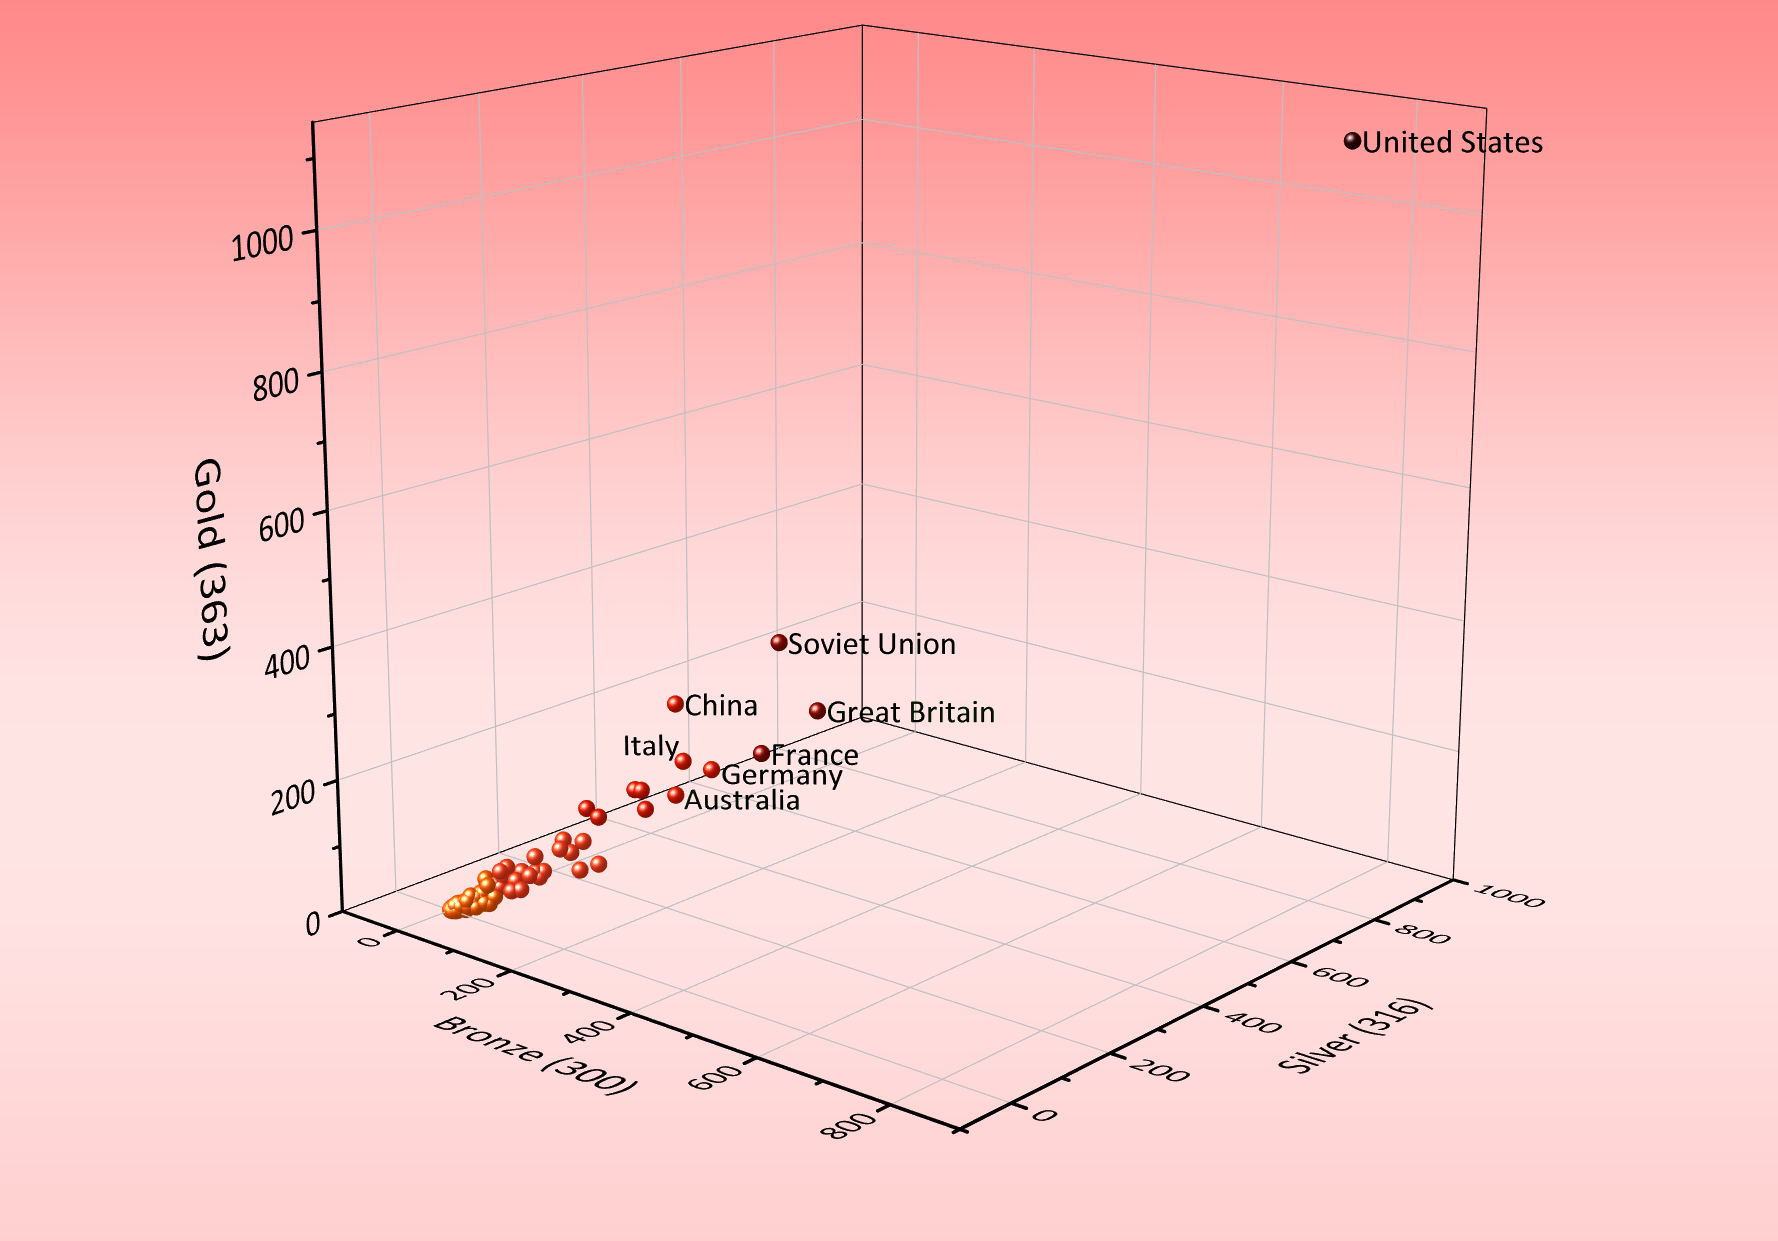
\includegraphics[width=\textwidth]{Level.png}
%	\caption{Flow Chart of Our Work}
%	\label{img}
%\end{figure}
	\caption{The result of Model 2}\label{fig:result}
\end{figure}

\begin{figure}[htbp]
	\centering
	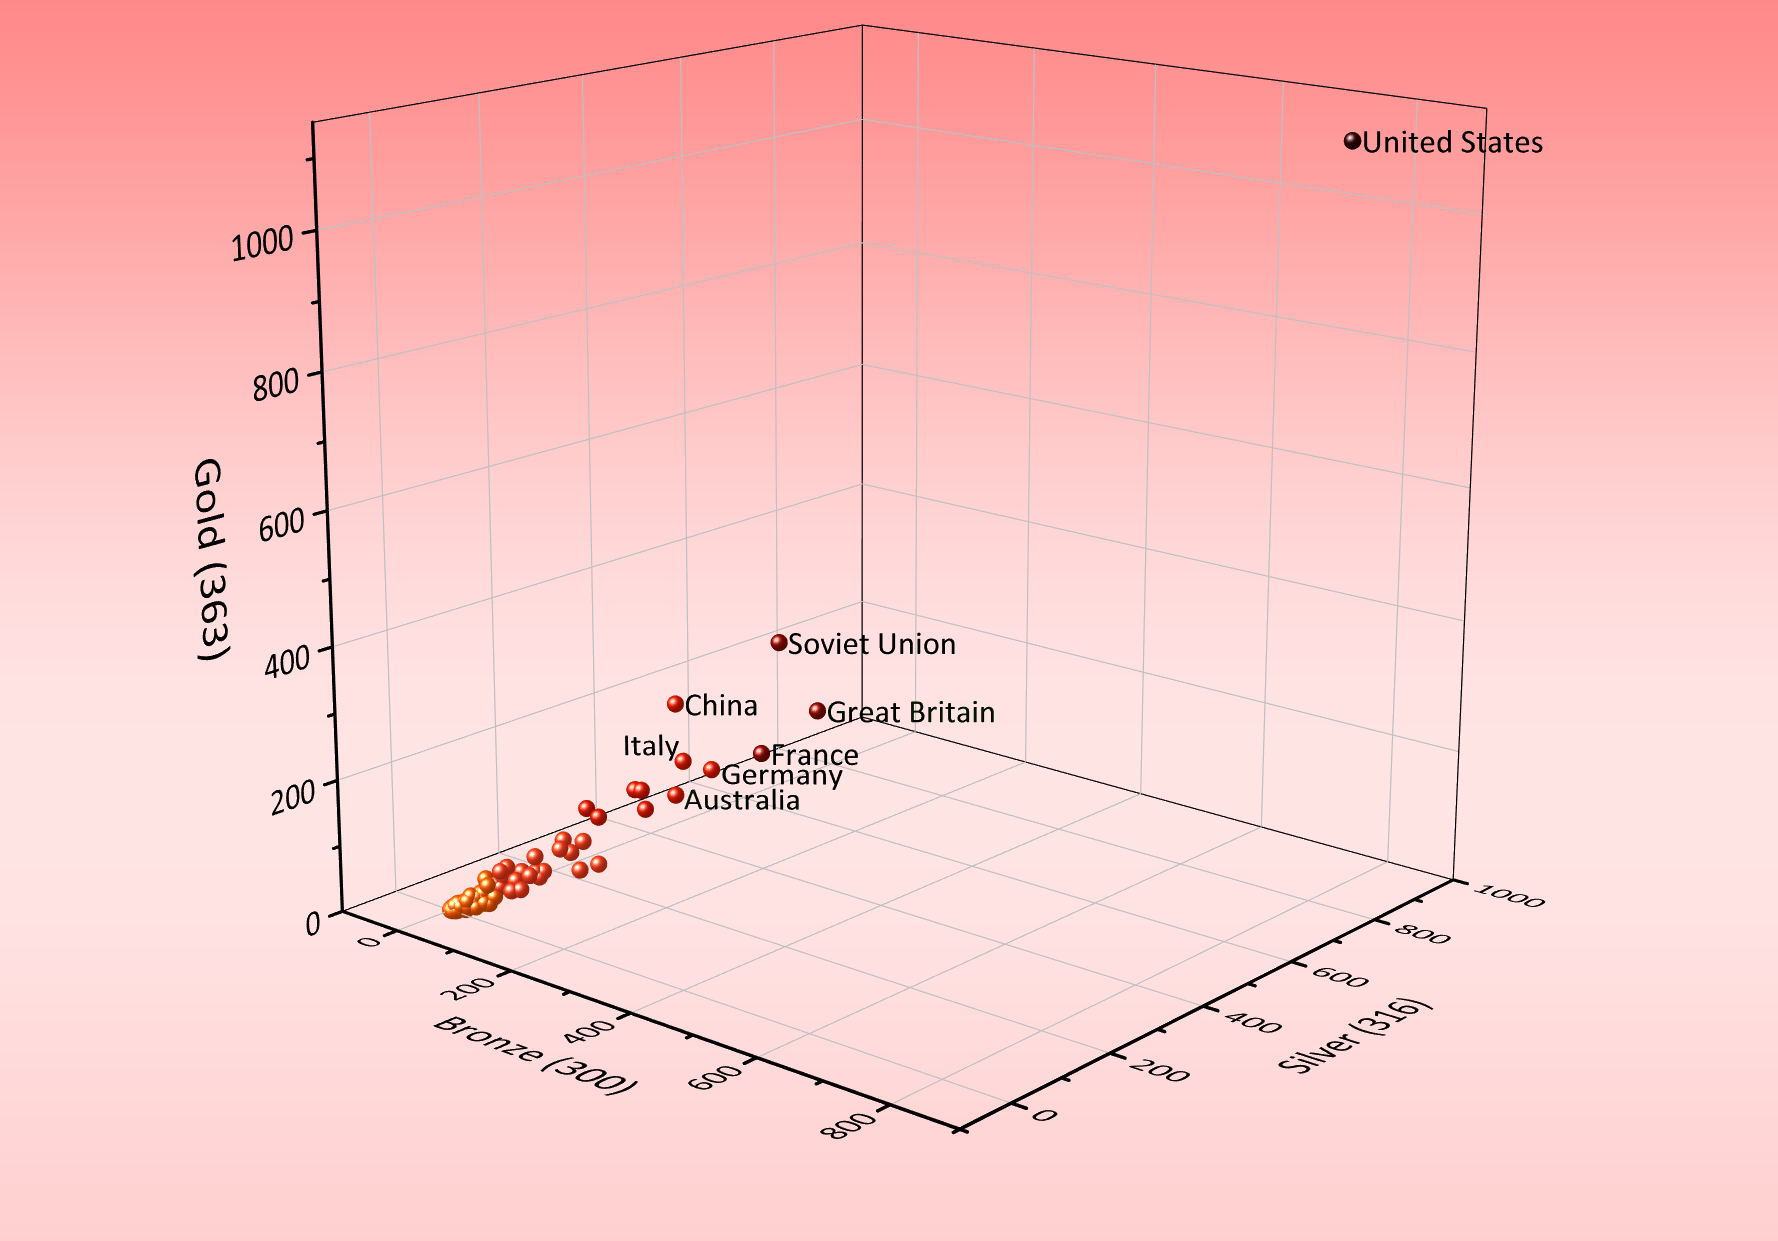
\includegraphics[width=\textwidth]{Level.png}
	%	\caption{Flow Chart of Our Work}
	%	\label{img}
	%\end{figure}
	\caption{The result of Model 2}\label{fig:result}
\end{figure}

\begin{figure}[htbp]
	\centering
	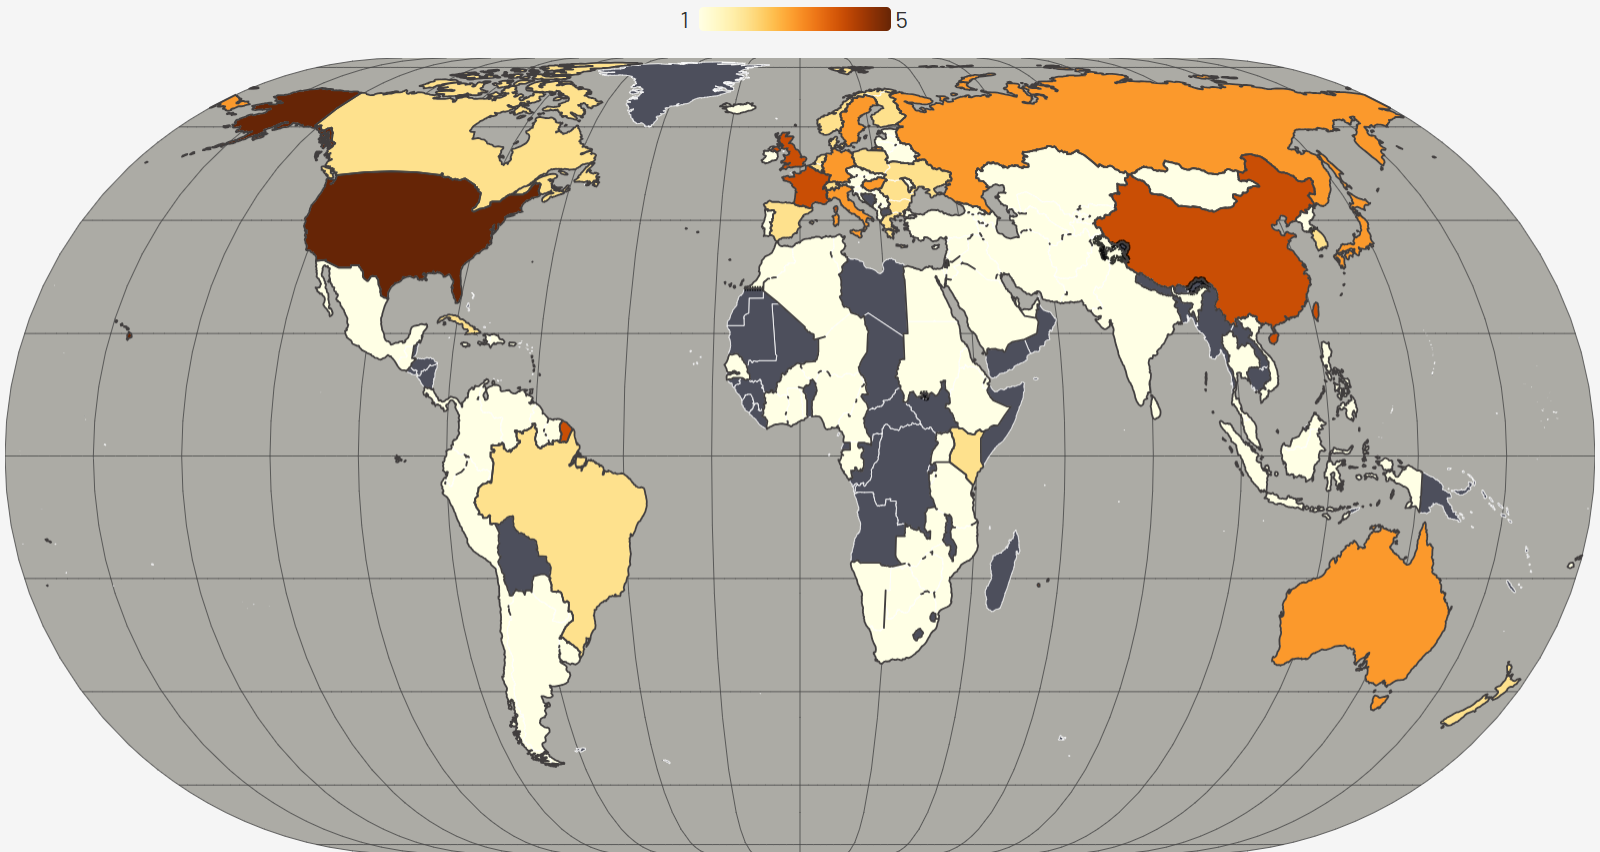
\includegraphics[width=12cm]{img/Level2.png}
	\caption{aa}
	\label{fig:aa}
\end{figure}


\begin{figure}[htbp]
	\centering
	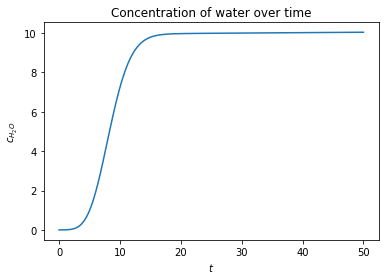
\includegraphics[width=.8\textwidth]{water.png}
	\caption{The result of Model 2}\label{fig:result}
\end{figure}
\begin{enumerate}[\bfseries 1.]
    \item We do ...
    \item We do ...
    \item We do ...
\end{enumerate}

\section{Assumptions}


\section{Notations}

The primary notations used in this paper are listed in Table \ref{tb:notation}.

% 三线表示例
\begin{table}[!htbp]
\begin{center}
\caption{Notations}
\begin{tabular}{cl}
	\toprule
	\multicolumn{1}{m{3cm}}{\centering Symbol}
	&\multicolumn{1}{m{8cm}}{\centering Definition}\\
	\midrule
	$A$&the first one\\
	$b$&the second one\\
	$\alpha$ &the last one\\
	$\sum m_{c_{i} S_{j}}$ &the last one\\
	\bottomrule
\end{tabular}\label{tb:notation}
\end{center}
\end{table}

\section{Data Preprocessing}
\subsection{Basic Data Preprocessing}
\subsection{Data Mining}
\section{Task1:}
\subsection{Details about Model 1}
The detail can be described by equation \eqref{eq1}:\autoref{eq1}:
%带标签的方程
\begin{equation}\label{eq1}
\alpha+\beta=\gamma
\end{equation}
%不带标签的方程
\[
\alpha+\beta=\gamma
\]
$$\alpha$$


%长等式
\begin{equation}\label{eq2}
	\begin{split}
	&A+B+C+D+E+F\\
	&=G+Q+W+E+R+T+Y\\
	&=A+S+D+F+G+H+J
	\end{split}
\end{equation}
%分段方程
\begin{equation}\label{eq3}
	F(x)=
	\begin{cases}
		0&,\text{if $x<0$}\\
		x+1&,\text{if $x>0$}\\
		1&,\text{otherwise}
			\end{cases}
\end{equation}

%Table 2 : Variable Name
\begin{longtblr}[
	caption = {Variable Name},
	]{
		vline{1-4} = {1-10}{},
		hline{1-11} = {1-3}{},
	}
	Variable Name                                                    & \textit{Code}                                                & Definition                                                                      &  \\
	Whether~Host Country                                             & \textit{is host}                                             & {Whether the country is the host(1 for host,0 for\\~non-host)}                  &  \\
	{Medal Expectation\\Increment *Personnel\\Expectation lncrement} & {\textit{medal\_increment *}\\\textit{personnel\_increment}} & {Product of medal\\expectation increment and\\personnel expectation\\increment} &  \\
	{Sport Advantage\\Coefficient}                                 & \textit{sport\_adv}                                           & {Advantage coefficient of\\a specific sport}                                  &  \\
	Country Level                                                    & \textit{country\_lvl}                                        & {The level of the country in the competition\\(ordered by rank)}                &  \\
	{Project Medal\\Expectation /Project\\Personnel Expection~}                         & \textit{sport\_medal \_per\_ person}                          & {Ratio of sport medals to projected personnel\\for a specific sport}          &  \\
	Gold Medal Probability                                           & \textit{gold\_prob}                                          & {Probability of an athlete~\\winning a gold medal}                              &  \\
	{Silver Medal\\Probability}                                      & \textit{silver\_prob}                                        & Probability of an athlete~ winning a silver medal                               &  \\
	{Bronze Medal\\Probability}                                      & \textit{silver\_prob}                                        & Probability of an athletewinning a bronze medal                                 &  \\
	No Medal Probability                                             & \textit{no\_medal\_probe}                                    & Probability of an athlete winning no medal                                      &  \\
	&                                                              &                                                                                 &  \\
	&                                                              &                                                                                 &  
\end{longtblr}


\section{Task2:}
\subsection{Conclusion of Model 2}
The results are shown in Figure \ref{fig:result}, where $t$ denotes the time in seconds, and $c$ refers to the concentration of water in the boiler.

\begin{figure}[htbp]
\centering
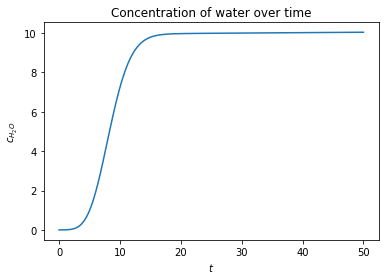
\includegraphics[width=.8\textwidth]{water.png}
\caption{The result of Model 2}\label{fig:result}
\end{figure}

\clearpage
\subsection{Commetary on Model 2}
The instance of long and wide tables are shown in Table \ref{tb:longtable}.

% 长表格示例,更多用法请参考 longtable 宏包文档
% 以下环境及对应参数可实现表格内的自动换行与表格的自动断页
% 您也可以选择自行载入 tabularx 宏包,并通过 X 参数指定对应列自动换行






Figure \ref{fig:subfigures} gives an example of subfigures. Figure \ref{subfig:left} is on the left, and Figure \ref{subfig:right} is on the right.

% 子图(多图并列)示例,更多用法请参考 subfigure 宏包文档
% 如果您只希望几张图并列,不需要额外的 caption,那么在 figure 环境中
% 连续插入总宽度不超过 \textwidth 的多个 \includegraphics 命令即可
\begin{figure}[htbp]
\centering
\begin{subfigure}[b]{.4\textwidth}
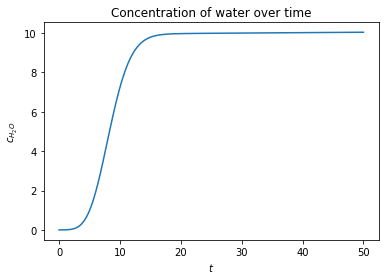
\includegraphics[width=\textwidth]{water.png}
\caption{Image on the left}\label{subfig:left}
\end{subfigure}
\begin{subfigure}[b]{.4\textwidth}
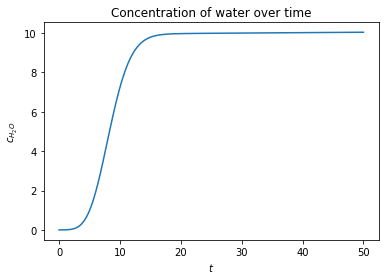
\includegraphics[width=\textwidth]{water.png}
\caption{Image on the right}\label{subfig:right}
\end{subfigure}
\caption{Two images}\label{fig:subfigures}
\end{figure}

\section{Task3}

\section{Task4}

\section{Sensitivity Analysis}

\section{Model Evaluation}
\subsection{Strengths}
\begin{itemize}
    \item First one...
    \item Second one ...
\end{itemize}

\subsection{Weaknesses}
\begin{itemize}
    \item Only one ...
 \end{itemize}
 
\section{Conclusion}

% 以下为信件/备忘录部分,不需要可自行去掉
% 如有需要可将整个 letter 环境移动到文章开头或中间
% 请在第二个花括号内填写标题,如「信件」(Letter)或「备忘录」(Memorandum)
\begin{letter}{Memorandum}
\begin{flushleft}  % 左对齐环境,无首行缩进
\textbf{To:} Heishan Yan\\
\textbf{From:} Team 1234567\\
\textbf{Date:} October 1st, 2019\\
\textbf{Subject:} A better choice than MS Word: \LaTeX
\end{flushleft}

In the memo, we want to introduce you an alternate typesetting program to the prevailing MS Word: \textbf{\LaTeX}. In fact, the history of \LaTeX\ is even longer than that of MS Word. In 1970s, the famous computer scientist Donald Knuth first came out with a typesetting program, which named \TeX\ \ldots

Firstly, \ldots

Secondly, \ldots

Lastly, \ldots

According to all those mentioned above, it is really worth to have a try on \LaTeX! 
\end{letter}


% 参考文献,此处以 MLA 引用格式为例
\begin{thebibliography}{99}
\bibitem{1} Einstein, A., Podolsky, B., \& Rosen, N. (1935). Can quantum-mechanical description of physical reality be considered complete?. \emph{Physical review}, 47(10), 777.
\bibitem{2} \emph{A simple, easy \LaTeX\ template for MCM/ICM: EasyMCM}. (2018). Retrieved December 1, 2019, from\url{https://www.cnblogs.com/xjtu-blacksmith/p/easymcm.html}
\end{thebibliography}


% 以下为附录内容
% 如您的论文中不需要附录,请自行删除
\begin{subappendices}  % 附录环境

\section{Appendix A: Further on \LaTeX}
To clarify the importance of using \LaTeX\ in MCM or ICM, several points need to be covered, which are \ldots

To be more specific, \ldots

All in all, \ldots

Anyway, nobody \textbf{really} needs such appendix \ldots

\section{Appendix B: Program Codes}
Here are the program codes we used in our research.

% 代码环境示例三则
% 如您的论文不需要展示代码,请删除
% 更多用法,请参考 listings 宏包文档

% Python 代码示例
\begin{lstlisting}[language=Python, name={test.py}]
# Python code example
for i in range(10):
    print('Hello, world!')
\end{lstlisting}

% MATLAB 代码示例
\begin{lstlisting}[language=MATLAB, name={test.m}]
% MATLAB code example
for i = 1:10
    disp("hello, world!");
end
\end{lstlisting}



% C++ 代码示例
\begin{lstlisting}[language=C++, name={test.cpp}]
// C++ code example
#include <iostream>
using namespace std;

int main() {
    for (int i = 0; i < 10; i++)
        cout << "hello, world" << endl;
    return 0;
}
\end{lstlisting}

\end{subappendices}  % 附录内容结束

\end{document}  % 结束
